
\begin{appendices}
%% Flight results
\chapter{C++ Simulation Complete Results}
\section{C++ Simulation SNR Profiles}\label{app:cSNRProfiles_all}
\begin{figure}[ht!]
\includegraphics{figures/c_sim_snr/EsNo_profile_1.eps}
\caption{SNR Profile number 1, used in C++ simulation.}
\end{figure}
\begin{figure}[ht!]
\includegraphics{figures/c_sim_snr/EsNo_profile_2.eps}
\caption{SNR Profile number 2, used in C++ simulation.}
\end{figure}
\begin{figure}[ht!]
\includegraphics{figures/c_sim_snr/EsNo_profile_3.eps}
\caption{SNR Profile number 3, used in C++ simulation.}
\end{figure}
\begin{figure}[ht!]
\includegraphics{figures/c_sim_snr/EsNo_profile_4.eps}
\caption{SNR Profile number 4, used in C++ simulation.}
\end{figure}
\begin{figure}[ht!]
\includegraphics{figures/c_sim_snr/EsNo_profile_5.eps}
\caption{SNR Profile number 5, used in C++ simulation.}
\end{figure}
\begin{figure}[ht!]
\includegraphics{figures/c_sim_snr/EsNo_profile_6.eps}
\caption{SNR Profile number 6, used in C++ simulation.}
\end{figure}
\begin{figure}[ht!]
\includegraphics{figures/c_sim_snr/EsNo_profile_7.eps}
\caption{SNR Profile number 7, used in C++ simulation.}
\end{figure}
\begin{figure}[ht!]
\includegraphics{figures/c_sim_snr/EsNo_profile_8.eps}
\caption{SNR Profile number 8, used in C++ simulation.}
\end{figure}
\begin{figure}[ht!]
\includegraphics{figures/c_sim_snr/EsNo_profile_9.eps}
\caption{SNR Profile number 9, used in C++ simulation.}
\end{figure}
\begin{figure}[ht!]
\includegraphics{figures/c_sim_snr/EsNo_profile_10.eps}
\caption{SNR Profile number 10, used in C++ simulation.}
\end{figure}
\begin{figure}[ht!]
\includegraphics{figures/c_sim_snr/EsNo_profile_11.eps}
\caption{SNR Profile number 11, used in C++ simulation. Result is ignored for the most part, but included in sum of binned mean plots, so is included in this appendix.}
\end{figure}
\begin{figure}[ht!]
\includegraphics{figures/c_sim_snr/EsNo_profile_12.eps}
\caption{SNR Profile number 12, used in C++ simulation.}
\end{figure}
\begin{figure}[ht!]
\includegraphics{figures/c_sim_snr/EsNo_profile_13.eps}
\caption{SNR Profile number 13, used in C++ simulation.}
\end{figure}
\begin{figure}[ht!]
\includegraphics{figures/c_sim_snr/EsNo_profile_14.eps}
\caption{SNR Profile number 14, used in C++ simulation.}
\end{figure}
\begin{figure}[ht!]
\includegraphics{figures/c_sim_snr/EsNo_profile_15.eps}
\caption{SNR Profile number 15, used in C++ simulation.}
\end{figure}
\begin{figure}[ht!]
\includegraphics{figures/c_sim_snr/EsNo_profile_16.eps}
\caption{SNR Profile number 16, used in C++ simulation.}
\end{figure}
\begin{figure}[ht!]
\includegraphics{figures/c_sim_snr/EsNo_profile_17.eps}
\caption{SNR Profile number 17, used in C++ simulation.}
\end{figure}
\begin{figure}[ht!]
\includegraphics{figures/c_sim_snr/EsNo_profile_18.eps}
\caption{SNR Profile number 18, used in C++ simulation.}
\end{figure}
\begin{figure}[ht!]
\includegraphics{figures/c_sim_snr/EsNo_profile_19.eps}
\caption{SNR Profile number 19, used in C++ simulation.}
\end{figure}
\begin{figure}[ht!]
\includegraphics{figures/c_sim_snr/EsNo_profile_20.eps}
\caption{SNR Profile number 20, used in C++ simulation.}
\end{figure}
\begin{figure}[ht!]
\includegraphics{figures/c_sim_snr/EsNo_profile_21.eps}
\caption{SNR Profile number 21, used in C++ simulation.}
\end{figure}
\begin{figure}[ht!]
\includegraphics{figures/c_sim_snr/EsNo_profile_22.eps}
\caption{SNR Profile number 22, used in C++ simulation.}
\end{figure}
\begin{figure}[ht!]
\includegraphics{figures/c_sim_snr/EsNo_profile_23.eps}
\caption{SNR Profile number 23, used in C++ simulation.}
\end{figure}
\begin{figure}[ht!]
\includegraphics{figures/c_sim_snr/EsNo_profile_24.eps}
\caption{SNR Profile number 24, used in C++ simulation.}
\end{figure}
\clearpage
\section{C++ Simulation Time Series}
\subsection{Power Saving Mission}
\begin{figure}[ht!]
\includegraphics{figures/c_sim_timeSeries/Fitness_timeSeries_LM_1.eps}
\includegraphics{figures/c_sim_timeSeries/Fitness_timeSeries_RLM_1.eps}
\includegraphics{figures/c_sim_timeSeries/Fitness_timeSeries_NSE_1.eps}
\caption{Time Series plots for SNR Profile number 1, using the Powersaving Mission. The first plot is from CE-LM, the second plot is from CE-RLM, the third plot is from CE-NSE.}
\end{figure}
\begin{figure}[ht!]
\includegraphics{figures/c_sim_timeSeries/Fitness_timeSeries_LM_2.eps}
\includegraphics{figures/c_sim_timeSeries/Fitness_timeSeries_RLM_2.eps}
\includegraphics{figures/c_sim_timeSeries/Fitness_timeSeries_NSE_2.eps}
\caption{Time Series plots for SNR Profile number 2, using the Powersaving Mission. The first plot is from CE-LM, the second plot is from CE-RLM, the third plot is from CE-NSE.}
\end{figure}
\begin{figure}[ht!]
\includegraphics{figures/c_sim_timeSeries/Fitness_timeSeries_LM_3.eps}
\includegraphics{figures/c_sim_timeSeries/Fitness_timeSeries_RLM_3.eps}
\includegraphics{figures/c_sim_timeSeries/Fitness_timeSeries_NSE_3.eps}
\caption{Time Series plots for SNR Profile number 3, using the Powersaving Mission. The first plot is from CE-LM, the second plot is from CE-RLM, the third plot is from CE-NSE.}
\end{figure}
\begin{figure}[ht!]
\includegraphics{figures/c_sim_timeSeries/Fitness_timeSeries_LM_4.eps}
\includegraphics{figures/c_sim_timeSeries/Fitness_timeSeries_RLM_4.eps}
\includegraphics{figures/c_sim_timeSeries/Fitness_timeSeries_NSE_4.eps}
\caption{Time Series plots for SNR Profile number 4, using the Powersaving Mission. The first plot is from CE-LM, the second plot is from CE-RLM, the third plot is from CE-NSE.}
\end{figure}
\begin{figure}[ht!]
\includegraphics{figures/c_sim_timeSeries/Fitness_timeSeries_LM_5.eps}
\includegraphics{figures/c_sim_timeSeries/Fitness_timeSeries_RLM_5.eps}
\includegraphics{figures/c_sim_timeSeries/Fitness_timeSeries_NSE_5.eps}
\caption{Time Series plots for SNR Profile number 5, using the Powersaving Mission. The first plot is from CE-LM, the second plot is from CE-RLM, the third plot is from CE-NSE.}
\end{figure}
\begin{figure}[ht!]
\includegraphics{figures/c_sim_timeSeries/Fitness_timeSeries_LM_6.eps}
\includegraphics{figures/c_sim_timeSeries/Fitness_timeSeries_RLM_6.eps}
\includegraphics{figures/c_sim_timeSeries/Fitness_timeSeries_NSE_6.eps}
\caption{Time Series plots for SNR Profile number 6, using the Powersaving Mission. The first plot is from CE-LM, the second plot is from CE-RLM, the third plot is from CE-NSE.}
\end{figure}
\begin{figure}[ht!]
\includegraphics{figures/c_sim_timeSeries/Fitness_timeSeries_LM_7.eps}
\includegraphics{figures/c_sim_timeSeries/Fitness_timeSeries_RLM_7.eps}
\includegraphics{figures/c_sim_timeSeries/Fitness_timeSeries_NSE_7.eps}
\caption{Time Series plots for SNR Profile number 7, using the Powersaving Mission. The first plot is from CE-LM, the second plot is from CE-RLM, the third plot is from CE-NSE.}
\end{figure}
\begin{figure}[ht!]
\includegraphics{figures/c_sim_timeSeries/Fitness_timeSeries_LM_8.eps}
\includegraphics{figures/c_sim_timeSeries/Fitness_timeSeries_RLM_8.eps}
\includegraphics{figures/c_sim_timeSeries/Fitness_timeSeries_NSE_8.eps}
\caption{Time Series plots for SNR Profile number 8, using the Powersaving Mission. The first plot is from CE-LM, the second plot is from CE-RLM, the third plot is from CE-NSE.}
\end{figure}
\begin{figure}[ht!]
\includegraphics{figures/c_sim_timeSeries/Fitness_timeSeries_LM_9.eps}
\includegraphics{figures/c_sim_timeSeries/Fitness_timeSeries_RLM_9.eps}
\includegraphics{figures/c_sim_timeSeries/Fitness_timeSeries_NSE_9.eps}
\caption{Time Series plots for SNR Profile number 9, using the Powersaving Mission. The first plot is from CE-LM, the second plot is from CE-RLM, the third plot is from CE-NSE.}
\end{figure}
\begin{figure}[ht!]
\includegraphics{figures/c_sim_timeSeries/Fitness_timeSeries_LM_10.eps}
\includegraphics{figures/c_sim_timeSeries/Fitness_timeSeries_RLM_10.eps}
\includegraphics{figures/c_sim_timeSeries/Fitness_timeSeries_NSE_10.eps}
\caption{Time Series plots for SNR Profile number 10, using the Powersaving Mission. The first plot is from CE-LM, the second plot is from CE-RLM, the third plot is from CE-NSE.}
\end{figure}
\begin{figure}[ht!]
\includegraphics{figures/c_sim_timeSeries/Fitness_timeSeries_LM_11.eps}
\includegraphics{figures/c_sim_timeSeries/Fitness_timeSeries_RLM_11.eps}
\includegraphics{figures/c_sim_timeSeries/Fitness_timeSeries_NSE_11.eps}
\caption{Time Series plots for SNR Profile number 11, using the Powersaving Mission. The first plot is from CE-LM, the second plot is from CE-RLM, the third plot is from CE-NSE.}
\end{figure}
\begin{figure}[ht!]
\includegraphics{figures/c_sim_timeSeries/Fitness_timeSeries_LM_12.eps}
\includegraphics{figures/c_sim_timeSeries/Fitness_timeSeries_RLM_12.eps}
\includegraphics{figures/c_sim_timeSeries/Fitness_timeSeries_NSE_12.eps}
\caption{Time Series plots for SNR Profile number 12, using the Powersaving Mission. The first plot is from CE-LM, the second plot is from CE-RLM, the third plot is from CE-NSE.}
\end{figure}
\begin{figure}[ht!]
\includegraphics{figures/c_sim_timeSeries/Fitness_timeSeries_LM_13.eps}
\includegraphics{figures/c_sim_timeSeries/Fitness_timeSeries_RLM_13.eps}
\includegraphics{figures/c_sim_timeSeries/Fitness_timeSeries_NSE_13.eps}
\caption{Time Series plots for SNR Profile number 13, using the Powersaving Mission. The first plot is from CE-LM, the second plot is from CE-RLM, the third plot is from CE-NSE.}
\end{figure}
\begin{figure}[ht!]
\includegraphics{figures/c_sim_timeSeries/Fitness_timeSeries_LM_14.eps}
\includegraphics{figures/c_sim_timeSeries/Fitness_timeSeries_RLM_14.eps}
\includegraphics{figures/c_sim_timeSeries/Fitness_timeSeries_NSE_14.eps}
\caption{Time Series plots for SNR Profile number 14, using the Powersaving Mission. The first plot is from CE-LM, the second plot is from CE-RLM, the third plot is from CE-NSE.}
\end{figure}
\begin{figure}[ht!]
\includegraphics{figures/c_sim_timeSeries/Fitness_timeSeries_LM_15.eps}
\includegraphics{figures/c_sim_timeSeries/Fitness_timeSeries_RLM_15.eps}
\includegraphics{figures/c_sim_timeSeries/Fitness_timeSeries_NSE_15.eps}
\caption{Time Series plots for SNR Profile number 15, using the Powersaving Mission. The first plot is from CE-LM, the second plot is from CE-RLM, the third plot is from CE-NSE.}
\end{figure}
\begin{figure}[ht!]
\includegraphics{figures/c_sim_timeSeries/Fitness_timeSeries_LM_16.eps}
\includegraphics{figures/c_sim_timeSeries/Fitness_timeSeries_RLM_16.eps}
\includegraphics{figures/c_sim_timeSeries/Fitness_timeSeries_NSE_16.eps}
\caption{Time Series plots for SNR Profile number 16, using the Powersaving Mission. The first plot is from CE-LM, the second plot is from CE-RLM, the third plot is from CE-NSE.}
\end{figure}
\begin{figure}[ht!]
\includegraphics{figures/c_sim_timeSeries/Fitness_timeSeries_LM_17.eps}
\includegraphics{figures/c_sim_timeSeries/Fitness_timeSeries_RLM_17.eps}
\includegraphics{figures/c_sim_timeSeries/Fitness_timeSeries_NSE_17.eps}
\caption{Time Series plots for SNR Profile number 17, using the Powersaving Mission. The first plot is from CE-LM, the second plot is from CE-RLM, the third plot is from CE-NSE.}
\end{figure}
\begin{figure}[ht!]
\includegraphics{figures/c_sim_timeSeries/Fitness_timeSeries_LM_18.eps}
\includegraphics{figures/c_sim_timeSeries/Fitness_timeSeries_RLM_18.eps}
\includegraphics{figures/c_sim_timeSeries/Fitness_timeSeries_NSE_18.eps}
\caption{Time Series plots for SNR Profile number 18, using the Powersaving Mission. The first plot is from CE-LM, the second plot is from CE-RLM, the third plot is from CE-NSE.}
\end{figure}
\begin{figure}[ht!]
\includegraphics{figures/c_sim_timeSeries/Fitness_timeSeries_LM_19.eps}
\includegraphics{figures/c_sim_timeSeries/Fitness_timeSeries_RLM_19.eps}
\includegraphics{figures/c_sim_timeSeries/Fitness_timeSeries_NSE_19.eps}
\caption{Time Series plots for SNR Profile number 19, using the Powersaving Mission. The first plot is from CE-LM, the second plot is from CE-RLM, the third plot is from CE-NSE.}
\end{figure}
\begin{figure}[ht!]
\includegraphics{figures/c_sim_timeSeries/Fitness_timeSeries_LM_20.eps}
\includegraphics{figures/c_sim_timeSeries/Fitness_timeSeries_RLM_20.eps}
\includegraphics{figures/c_sim_timeSeries/Fitness_timeSeries_NSE_20.eps}
\caption{Time Series plots for SNR Profile number 20, using the Powersaving Mission. The first plot is from CE-LM, the second plot is from CE-RLM, the third plot is from CE-NSE.}
\end{figure}
\begin{figure}[ht!]
\includegraphics{figures/c_sim_timeSeries/Fitness_timeSeries_LM_21.eps}
\includegraphics{figures/c_sim_timeSeries/Fitness_timeSeries_RLM_21.eps}
\includegraphics{figures/c_sim_timeSeries/Fitness_timeSeries_NSE_21.eps}
\caption{Time Series plots for SNR Profile number 21, using the Powersaving Mission. The first plot is from CE-LM, the second plot is from CE-RLM, the third plot is from CE-NSE.}
\end{figure}
\begin{figure}[ht!]
\includegraphics{figures/c_sim_timeSeries/Fitness_timeSeries_LM_22.eps}
\includegraphics{figures/c_sim_timeSeries/Fitness_timeSeries_RLM_22.eps}
\includegraphics{figures/c_sim_timeSeries/Fitness_timeSeries_NSE_22.eps}
\caption{Time Series plots for SNR Profile number 22, using the Powersaving Mission. The first plot is from CE-LM, the second plot is from CE-RLM, the third plot is from CE-NSE.}
\end{figure}
\begin{figure}[ht!]
\includegraphics{figures/c_sim_timeSeries/Fitness_timeSeries_LM_23.eps}
\includegraphics{figures/c_sim_timeSeries/Fitness_timeSeries_RLM_23.eps}
\includegraphics{figures/c_sim_timeSeries/Fitness_timeSeries_NSE_23.eps}
\caption{Time Series plots for SNR Profile number 23, using the Powersaving Mission. The first plot is from CE-LM, the second plot is from CE-RLM, the third plot is from CE-NSE.}
\end{figure}
\begin{figure}[ht!]
\includegraphics{figures/c_sim_timeSeries/Fitness_timeSeries_LM_24.eps}
\includegraphics{figures/c_sim_timeSeries/Fitness_timeSeries_RLM_24.eps}
\includegraphics{figures/c_sim_timeSeries/Fitness_timeSeries_NSE_24.eps}
\caption{Time Series plots for SNR Profile number 24, using the Powersaving Mission. The first plot is from CE-LM, the second plot is from CE-RLM, the third plot is from CE-NSE.}
\end{figure}
\clearpage

\subsection{Emergency Mission}
\subsection{Cooperation Mission}
\textbf{\textit{[I'm not sure about doing this for all of them because it's going to take way too many pages - Max]}}
\section{Two-Dimension Histograms on C++ Simulation}\label{app:2dHistSim}
\par stub for 2dhists with sim.
\par \textbf{\textit{[holding off on these figures until I get a response about if I should use all of the figures. - Max]}}
\section{C++ Simulation Binned Mean Plots}
\par stub for C++ simulation binned mean plots. \par \textbf{\textit{[holding off on these figures until I get a response about if I should use all of the figures. - Max]}}
%% Test Results
\chapter{Flight Test Profiles}\label{app:flightSNRProfiles_all}
\par stub for Flight Test SNR profiles.
\section{Flight Test Time Series}
\section{Two-Dimension Histograms on Flight Test}\label{app:2dHistFlight}
\par stub for 2dhists with sim.
\section{Flight Test Binned Mean Plots}
\par stub for Flight Test binned mean plots


% \chapter{MATLAB Code}\label{app:MatlabCode}
% \section{Preface}
% \textit{\textbf{[The three CE implementations can probably be collapsed into one file - Max]}}
% \section{log\_parser.m}\label{app:MatlabCode:parser}
% \lstinputlisting[language=matlab]{code/MATLAB/log_parser.m}
% \clearpage
% \section{findTheoreticalBestAction.m}\label{app:MatlabCode:optimalCalc}
% \lstinputlisting[language=matlab]{code/MATLAB/findTheoreticalBestAction.m}
% \clearpage
% \section{CE-LM MATLAB Simulation}
% \lstinputlisting[language=matlab]{code/MATLAB/SCaN_v3.m}
% \clearpage
% \section{CE-RLM MATLAB Simulation}
% \lstinputlisting[language=matlab]{code/MATLAB/SCaN_rlm_v1_mhli.m}
% \clearpage
% \section{CE-NSE MATLAB Simulation}
% \lstinputlisting[language=matlab]{code/MATLAB/SCaN_learnNSE_mlp_mhli.m}
% \clearpage
% \section{RecurseMatrix.m}\label{app:MatlabCode:recurseMatrix}
% \lstinputlisting[language=matlab]{code/MATLAB/RecurseMatrix.m}
% \clearpage
% \section{decision\_ensemble.m}\label{app:MatlabCode:decisionEnsemble}
% \lstinputlisting[language=matlab]{code/MATLAB/decision_ensemble.m}
% \clearpage
% \section{learn\_nse\_update.m}\label{app:MatlabCode:learnNSEUpdate}
% \lstinputlisting[language=matlab]{code/MATLAB/learn_nse_update.m}
% \clearpage
% \section{mse\_reg.m}\label{app:MatlabCode:mseReg}
% \lstinputlisting[language=matlab]{code/MATLAB/mse_reg.m}
% \section{regress\_ensemble.m}\label{app:MatlabCode:regressEnsemble}
% \lstinputlisting[language=matlab]{code/MATLAB/regress_ensemble.m}
% \clearpage
% \section{rlm\_update.m}\label{app:MatlabCode:rlmUpdate}
% \lstinputlisting[language=matlab]{code/MATLAB/rlm_update.m}
% \clearpage
% \section{trainrlm.m}\label{app:MatlabCode:trainrlm}
% \lstinputlisting[language=matlab]{code/MATLAB/trainrlm.m}
% \clearpage

% \chapter{C++ Code} \label{app:CppCode}
% \section{RLNNCognitiveEngineTester\_V3.cpp}\label{app:CppCode:cogEngTesterV3}
% \lstinputlisting[language=C++]{code/C++/RLNNCognitiveEngineTester_v3.cpp}
% \clearpage
% \section{RLNNCognitiveEngine.cpp}\label{app:CppCode:cogEng}
% \lstinputlisting[language=C++]{code/C++/RLNNCognitiveEngine.cpp}
% \clearpage
% \section{NeuralNetworkPredictor.cpp}\label{app:CppCode:nnPredictor}
% \lstinputlisting[language=C++]{code/C++/NeuralNetworkPredictor.cpp}
% \clearpage
% \section{LearnNSEPredictor.cpp} \label{app:CppCode:LearnNSE}
% \lstinputlisting[language=C++]{code/C++/LearnNSEPredictor.cpp}
% \clearpage
% \section{FeedForwardNeuralNetwork.cpp} \label{app:CppCode:ffnn}
% \lstinputlisting[language=C++]{code/C++/FeedForwardNetwork.cpp}
% \clearpage
% \section{TrainingDataBuffer.cpp} \label{app:CppCode:trainData}
% \lstinputlisting[language=C++]{code/C++/TrainingDataBuffer.cpp}
% \clearpage
% \section{ApplicationSpecificHelper.cpp} \label{app:CppCode:appSpecObj}
% \lstinputlisting[language=C++]{code/C++/ApplicationSpecificHelper.cpp}
% \clearpage
% \section{ThreeLayerNetwork.cpp} \label{app:CppCode:threeLayer}
% \lstinputlisting[language=C++]{code/C++/ThreeLayerNetwork.cpp}
% \clearpage
% \section{TwoLayerNetwork.cpp} \label{app:CppCode:twoLayer}
% \lstinputlisting[language=C++]{code/C++/TwoLayerNetwork.cpp}
% \clearpage
% \section{identity\_output\_layer.hpp} \label{app:CppCode:identityOutput}
% \lstinputlisting[language=C++]{code/C++/identity_output_layer.hpp}
% \clearpage
% \section{MemoryManagement.hpp} \label{app:CppCode:memManage}
% \lstinputlisting[language=C++]{code/C++/MemoryManagement.hpp}
% \clearpage
% \section{RecursiveLMHelper.cpp} \label{app:CppCode:rlmHelper}
% \lstinputlisting[language=C++]{code/C++/RecursiveLMHelper.cpp}
% \clearpage
% \section{Logging.hpp} \label{app:CppCode:loggingh}
% \lstinputlisting[language=C++]{code/C++/Logging.hpp}
% \clearpage
% \section{Logging.cpp} \label{app:CppCode:loggingc}
% \lstinputlisting[language=C++]{code/C++/Logging.cpp}
% \clearpage
% \section{Makefile} \label{app:CppCode:make}
% \lstinputlisting{code/C++/Makefile.txt}
% \clearpage


% \chapter{Pass Details, 2017}
% \par \textbf{\textit{[make this table actually ok]}}
% \par stub for pass details, 2017
% \chapter{Pass Details, 2018}
% \par \textbf{\textit{[make this table actually ok]}}
% \par \csvautotabular{2018_CE_Flight_test_passes.csv}



\end{appendices}